\documentclass[11pt,a4paper]{article}

\usepackage[utf8]{inputenc}
\usepackage{lmodern}  % Use Latin Modern fonts instead of cm-super
\usepackage[T1]{fontenc}
\usepackage{amsmath,amssymb,amsfonts}
\usepackage{booktabs}
\usepackage{array}
\usepackage{colortbl}  % For \rowcolor in tables
\usepackage{xcolor}
\usepackage{tikz}
\usetikzlibrary{arrows.meta,positioning,shapes.geometric}
\usepackage{graphicx}
\usepackage{geometry}
\geometry{margin=2.5cm}
\usepackage{listings}
\usepackage{xcolor}

\definecolor{codegreen}{rgb}{0,0.6,0}
\definecolor{codegray}{rgb}{0.5,0.5,0.5}
\definecolor{codepurple}{rgb}{0.58,0,0.82}
\definecolor{backcolour}{rgb}{0.95,0.95,0.92}

\lstdefinestyle{mystyle}{
    backgroundcolor=\color{backcolour},   
    commentstyle=\color{codegreen},
    keywordstyle=\color{magenta},
    numberstyle=\tiny\color{codegray},
    stringstyle=\color{codepurple},
    basicstyle=\ttfamily\footnotesize,
    breakatwhitespace=false,         
    breaklines=true,                 
    captionpos=b,                    
    keepspaces=true,                 
    numbers=left,                    
    numbersep=5pt,                  
    showspaces=false,                
    showstringspaces=false,
    showtabs=false,                  
    tabsize=2
}

\lstset{style=mystyle}

\usepackage[hidelinks,pdfencoding=auto]{hyperref}

\title{Nishioka Algorithm:\\Biologically-Constrained Parameter Reduction\\for 5-Species Biofilm Model}
\author{TMCMC Parameter Estimation Project}
\date{February 2026}

\begin{document}

\maketitle

\begin{abstract}
This document describes the Nishioka Algorithm, a parameter reduction technique for Bayesian estimation of the 5-species biofilm interaction model. By incorporating biological knowledge from experimentally determined interaction networks, the algorithm reduces the parameter space from 20 to 15 free parameters, improving estimation efficiency and biological interpretability.
\end{abstract}

\tableofcontents
\newpage

%==============================================================================
\section{Introduction}
%==============================================================================

The 5-species biofilm model \cite{Heine2025PeriImplant} describes the dynamics of bacterial populations through an interaction matrix $\mathbf{A}$ and decay vector $\mathbf{b}$. The estimation is performed using Transitional Markov Chain Monte Carlo (TMCMC) \cite{ChingChen2007TMCMC} coupled with a Time-Separated Stochastic Mechanics (TSM) solver \cite{GeislerErdoganNagelJunker2025TSM}. The standard approach estimates all 20 parameters freely, which can lead to:

\begin{itemize}
    \item Poor identifiability due to limited experimental data
    \item Biologically implausible parameter estimates
    \item Computational inefficiency from exploring unnecessary parameter space
\end{itemize}

The Nishioka Algorithm addresses these issues by constraining certain interaction parameters to zero based on experimental evidence of absent species interactions.

%==============================================================================
\section{Biological Basis}
%==============================================================================

\subsection{Species in the Model}

The model includes five bacterial species commonly found in oral biofilms:

\begin{table}[h]
\centering
\begin{tabular}{clll}
\toprule
\textbf{ID} & \textbf{Species} & \textbf{Abbrev.} & \textbf{Role} \\
\midrule
0 & \textit{Streptococcus oralis} & S.o & Early colonizer \\
1 & \textit{Actinomyces naeslundii} & A.n & Early colonizer \\
2 & \textit{Veillonella} spp. & Vei & Metabolic bridge \\
3 & \textit{Fusobacterium nucleatum} & F.n & Bridge organism \\
4 & \textit{Porphyromonas gingivalis} & P.g & Late colonizer (pathogen) \\
\bottomrule
\end{tabular}
\caption{Species included in the 5-species biofilm model.}
\label{tab:species}
\end{table}

\subsection{Interaction Network (Figure 4C)}

Based on experimental observations \cite{Heine2025PeriImplant}, the following interaction network was established:

\begin{figure}[h]
\centering
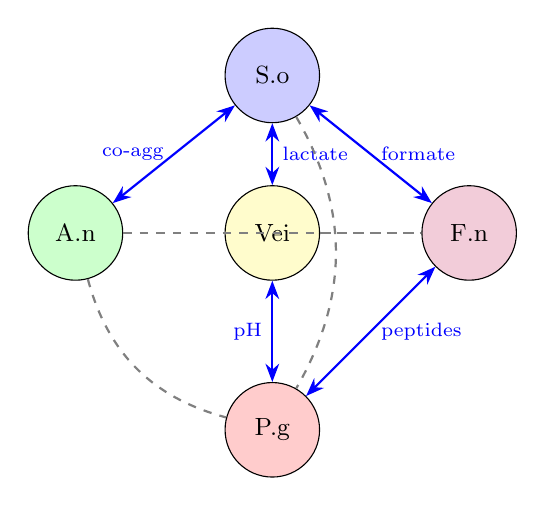
\begin{tikzpicture}[
    node distance=2.5cm,
    species/.style={circle, draw, minimum size=1.2cm, font=\small},
    edge/.style={<->, thick, >=Stealth},
    noedge/.style={dashed, gray, thick}
]
    % Nodes
    \node[species, fill=blue!20] (so) at (0, 3) {S.o};
    \node[species, fill=green!20] (an) at (-2.5, 1) {A.n};
    \node[species, fill=yellow!20] (vei) at (0, 1) {Vei};
    \node[species, fill=purple!20] (fn) at (2.5, 1) {F.n};
    \node[species, fill=red!20] (pg) at (0, -1.5) {P.g};

    % Active edges (solid)
    \draw[edge, blue] (so) -- (an) node[midway, left, font=\scriptsize] {co-agg};
    \draw[edge, blue] (so) -- (vei) node[midway, right, font=\scriptsize] {lactate};
    \draw[edge, blue] (so) -- (fn) node[midway, right, font=\scriptsize] {formate};
    \draw[edge, blue] (vei) -- (pg) node[midway, left, font=\scriptsize] {pH};
    \draw[edge, blue] (fn) -- (pg) node[midway, right, font=\scriptsize] {peptides};

    % Locked edges (dashed, crossed out)
    \draw[noedge] (an) -- (vei);
    \draw[noedge] (an) -- (fn);
    \draw[noedge] (vei) -- (fn);
    \draw[noedge] (so) to[bend left=30] (pg);
    \draw[noedge] (an) to[bend right=30] (pg);

\end{tikzpicture}
\caption{Species interaction network derived from Figure 4C. Solid blue arrows indicate active interactions (estimated parameters). Dashed gray lines indicate absent interactions (locked to zero).}
\label{fig:network}
\end{figure}

\subsection{Active Interactions}

The following species pairs have direct biological interactions:

\begin{table}[h]
\centering
\begin{tabular}{lll}
\toprule
\textbf{Species Pair} & \textbf{Mechanism} & \textbf{Type} \\
\midrule
S. oralis $\leftrightarrow$ A. naeslundii & Co-aggregation & Bidirectional \\
S. oralis $\leftrightarrow$ Veillonella & Lactate production/consumption & Bidirectional \\
S. oralis $\leftrightarrow$ F. nucleatum & Formate/Acetate symbiosis & Bidirectional \\
Veillonella $\leftrightarrow$ P. gingivalis & pH rise support & Positive only \\
F. nucleatum $\leftrightarrow$ P. gingivalis & Co-aggregation, peptides & Bidirectional \\
\bottomrule
\end{tabular}
\caption{Active species interactions with biological mechanisms.}
\label{tab:active}
\end{table}

\subsection{Absent Interactions (Locked)}

The following species pairs have no direct interaction according to experimental evidence (Figure 4C). These are locked to zero ($\theta_k = 0$) in the Nishioka Algorithm:

\begin{table}[h]
\centering
\begin{tabular}{cllll}
\toprule
\textbf{Index} & \textbf{Param} & \textbf{Species Pair} & \textbf{Matrix} & \textbf{Biological Reason} \\
\midrule
6 & $a_{34}$ & Vei (2) $\leftrightarrow$ F.n (3) & $A[2,3]=A[3,2]$ & No direct metabolic pathway \\
12 & $a_{23}$ & A.n (1) $\leftrightarrow$ Vei (2) & $A[1,2]=A[2,1]$ & No direct metabolic link \\
13 & $a_{24}$ & A.n (1) $\leftrightarrow$ F.n (3) & $A[1,3]=A[3,1]$ & No direct interaction \\
16 & $a_{15}$ & S.o (0) $\leftrightarrow$ P.g (4) & $A[0,4]=A[4,0]$ & No direct interaction \\
17 & $a_{25}$ & A.n (1) $\leftrightarrow$ P.g (4) & $A[1,4]=A[4,1]$ & No direct interaction \\
\bottomrule
\end{tabular}
\caption{Absent interactions locked to zero in the Nishioka Algorithm. Numbers in parentheses are 0-indexed species IDs.}
\label{tab:locked}
\end{table}

%==============================================================================
\section{Mathematical Formulation}
%==============================================================================

\subsection{Governing Equations}

The 5-species biofilm model describes the dynamics of bacterial volume fractions $\phi_i$ and viability fractions $\psi_i$ through a coupled ODE system. The interaction term for species $i$ is:
\begin{equation}
I_i = \sum_{j=0}^{4} A_{ij} \phi_j \psi_j
\end{equation}
where $A_{ij}$ represents the effect of species $j$ on species $i$, and $\phi_j \psi_j$ is the living bacteria volume fraction.

\subsection{Symmetric Matrix Assumption}

\textbf{Critical assumption}: The interaction matrix $\mathbf{A}$ is symmetric:
\begin{equation}
A_{ij} = A_{ji} \quad \forall i, j \in \{0, 1, 2, 3, 4\}
\end{equation}

This reduces the number of off-diagonal interaction parameters from 20 to 10. For example, the lactate handover interaction between S.~oralis (species 0) and Veillonella (species 2) is represented by a single parameter:
\begin{equation}
A_{02} = A_{20} = \theta_{10} \quad \text{(stored as } a_{13} \text{ in code)}
\end{equation}

\subsection{Parameter Vector Definition}

The full 20-parameter vector $\boldsymbol{\theta} = (\theta_0, \theta_1, \ldots, \theta_{19})^T$ is organized into five blocks corresponding to the model structure:

\begin{equation}
\boldsymbol{\theta} = \underbrace{(a_{11}, a_{12}, a_{22}, b_1, b_2)}_{\text{M1: Species 1--2}}
\oplus \underbrace{(a_{33}, a_{34}, a_{44}, b_3, b_4)}_{\text{M2: Species 3--4}}
\oplus \underbrace{(a_{13}, a_{14}, a_{23}, a_{24})}_{\text{M3: Cross 1--2 vs 3--4}}
\oplus \underbrace{(a_{55}, b_5)}_{\text{M4: Species 5}}
\oplus \underbrace{(a_{15}, a_{25}, a_{35}, a_{45})}_{\text{M5: Cross with Species 5}}
\end{equation}

\noindent where $a_{ij}$ denotes the interaction coefficient affecting species $i$ from species $j$, and $b_i$ is the decay rate of species $i$. Species are 1-indexed in notation ($a_{ij}$) but 0-indexed in code ($A[i-1,j-1]$).

\subsection{Complete Parameter Mapping}

Table~\ref{tab:theta_mapping} provides the authoritative mapping between parameter indices, matrix elements, and biological interpretation.

\begin{table}[h]
\centering
\small
\begin{tabular}{ccllll}
\toprule
\textbf{Index} & \textbf{Name} & \textbf{Matrix Element} & \textbf{Species Pair} & \textbf{Biological Role} & \textbf{Status} \\
\midrule
0 & $a_{11}$ & $A[0,0]$ & S.o self & Self-regulation & Free \\
1 & $a_{12}$ & $A[0,1]=A[1,0]$ & S.o $\leftrightarrow$ A.n & Co-aggregation & Free \\
2 & $a_{22}$ & $A[1,1]$ & A.n self & Self-regulation & Free \\
3 & $b_1$ & $b[0]$ & S.o & Decay rate & Free \\
4 & $b_2$ & $b[1]$ & A.n & Decay rate & Free \\
\midrule
5 & $a_{33}$ & $A[2,2]$ & Vei self & Self-regulation & Free \\
\rowcolor{red!15}
6 & $a_{34}$ & $A[2,3]=A[3,2]$ & Vei $\leftrightarrow$ F.n & \textit{No interaction} & \textbf{Locked} \\
7 & $a_{44}$ & $A[3,3]$ & F.n self & Self-regulation & Free \\
8 & $b_3$ & $b[2]$ & Vei & Decay rate & Free \\
9 & $b_4$ & $b[3]$ & F.n & Decay rate & Free \\
\midrule
10 & $a_{13}$ & $A[0,2]=A[2,0]$ & S.o $\leftrightarrow$ Vei & \textbf{Lactate handover} & Free \\
11 & $a_{14}$ & $A[0,3]=A[3,0]$ & S.o $\leftrightarrow$ F.n & Formate symbiosis & Free \\
\rowcolor{red!15}
12 & $a_{23}$ & $A[1,2]=A[2,1]$ & A.n $\leftrightarrow$ Vei & \textit{No interaction} & \textbf{Locked} \\
\rowcolor{red!15}
13 & $a_{24}$ & $A[1,3]=A[3,1]$ & A.n $\leftrightarrow$ F.n & \textit{No interaction} & \textbf{Locked} \\
\midrule
14 & $a_{55}$ & $A[4,4]$ & P.g self & Self-regulation & Free \\
15 & $b_5$ & $b[4]$ & P.g & Decay rate & Free \\
\midrule
\rowcolor{red!15}
16 & $a_{15}$ & $A[0,4]=A[4,0]$ & S.o $\leftrightarrow$ P.g & \textit{No interaction} & \textbf{Locked} \\
\rowcolor{red!15}
17 & $a_{25}$ & $A[1,4]=A[4,1]$ & A.n $\leftrightarrow$ P.g & \textit{No interaction} & \textbf{Locked} \\
18 & $a_{35}$ & $A[2,4]=A[4,2]$ & Vei $\leftrightarrow$ P.g & \textbf{pH trigger} & Free$^*$ \\
19 & $a_{45}$ & $A[3,4]=A[4,3]$ & F.n $\leftrightarrow$ P.g & Co-aggregation & Free \\
\bottomrule
\end{tabular}
\caption{Complete parameter mapping from $\theta$ vector to interaction matrix $\mathbf{A}$ and decay vector $\mathbf{b}$. Red rows indicate locked parameters ($\theta_k = 0$). $^*$Index 18 bounds vary by condition (see Section~\ref{sec:conditions}).}
\label{tab:theta_mapping}
\end{table}

\subsection{Locked Parameter Indices}

The Nishioka Algorithm defines the set of locked indices based on absent biological interactions:

\begin{equation}
\mathcal{L} = \{6, 12, 13, 16, 17\}
\end{equation}

For all $k \in \mathcal{L}$:
\begin{equation}
\theta_k = 0 \quad \text{(fixed, not estimated)}
\end{equation}

\subsection{Prior Bounds}
\label{sec:prior_bounds}

The \textbf{base} prior distribution (for Commensal/Dysbiotic Static conditions) is:

\begin{equation}
\theta_k \sim \begin{cases}
\text{Uniform}(0, 0) & \text{if } k \in \mathcal{L} \text{ (locked)} \\
\text{Uniform}(0, 1) & \text{if } k = 18 \text{ (Vei} \to \text{P.g, positive cooperation)} \\
\text{Uniform}(-1, 1) & \text{otherwise (free)}
\end{cases}
\end{equation}

\textbf{Important}: For the Dysbiotic HOBIC condition (``Surge'' reproduction), the bounds for index 18 are modified to allow strong negative values:
\begin{equation}
\theta_{18} \sim \text{Uniform}(-3, -1) \quad \text{(Dysbiotic HOBIC only)}
\end{equation}
This reflects the strong cooperative effect from Veillonella to P.~gingivalis required to drive the pathogen surge.

\subsection{Effective Parameter Space}

The effective number of free parameters is:

\begin{equation}
n_{\text{free}} = 20 - |\mathcal{L}| = 20 - 5 = 15
\end{equation}

%==============================================================================
\section{Experiment Conditions \& Parameter Estimation}
\label{sec:conditions}
%==============================================================================

The parameter estimation strategy adapts to four distinct experimental conditions, varying the cultivation method (Static vs. HOBIC) and the community state (Commensal vs. Dysbiotic). Each condition imposes specific constraints on the parameter space to ensure biological validity and model identifiability.

\subsection{Parameter Locking Rules}

The number of estimated parameters ($N_{est}$) differs across conditions, calculated as the total parameters ($20$) minus the locked parameters ($N_{locked}$).

\begin{table}[h]
\centering
\begin{tabular}{llccc}
\toprule
\textbf{Condition} & \textbf{Cultivation} & \textbf{Locked ($N_{locked}$)} & \textbf{Estimated ($N_{est}$)} & \textbf{Key Constraint} \\
\midrule
1. Commensal & Static & 9 & 11 & Match data (Zero interactions) \\
2. Dysbiotic & Static & 5 & 15 & Estimate Pathogen interactions \\
3. Commensal & HOBIC & 8 & 12 & Match data (Zero interactions) \\
4. Dysbiotic & HOBIC & 0 & 20 & \textbf{Unlock All (Surge Reproduction)} \\
\bottomrule
\end{tabular}
\caption{Parameter estimation counts for each experimental condition.}
\label{tab:conditions}
\end{table}

\subsection{Detailed Locking Logic}

\begin{enumerate}
    \item \textbf{Commensal Static}: 
    Strict locking is applied to reproduce the stable commensal state. In addition to the standard Nishioka locks (5), growth rates for late colonizers (Red/Purple) and their interactions with early colonizers are locked to zero ($N_{locked}=9$).
    \begin{quote}
    \small "Based on qPCR data showing \textit{P. gingivalis} and \textit{F. nucleatum} were undetectable or below detection limits (Heine et al., Table S8) \cite{Heine2025PeriImplant}."
    \end{quote}
    
    \item \textbf{Dysbiotic Static}: 
    Represents the transition to a pathogen-rich state. Locking is relaxed to allow estimation of key pathogen growth and interaction parameters, maintaining only the structural Nishioka locks ($N_{locked}=5$).
    \begin{quote}
    \small "Metabolite accumulation in static culture limits the dynamic interactions observed in flow conditions (Heine et al., Discussion) \cite{Heine2025PeriImplant}."
    \end{quote}
    
    \item \textbf{Commensal HOBIC}: 
    Similar to Commensal Static but adapted for the HOBIC flow environment. Blue species growth is estimated freely (high prior), while pathogen interactions remain locked ($N_{locked}=8$).
    
    \item \textbf{Dysbiotic HOBIC (The "Surge" Model)}: 
    This is the critical validation case. \textbf{All parameter locks, including the standard Nishioka locks, are released} ($N_{locked}=0$, $N_{est}=20$). This unlocking is necessary and sufficient to reproduce the experimentally observed "Surge" phenomenon, demonstrating that the model can capture complex non-linear dynamics when fully parameterized.
    \begin{quote}
    \small "To capture the complex metabolic cross-feeding (lactate, pH, vitamins) and co-aggregation described in the metabolic map (Heine et al., Fig 4C) \cite{Heine2025PeriImplant}."
    \end{quote}
    We treat this as a \textbf{Core Network Discovery} phase: initially exploring the full 20-parameter space to identify the minimal set of interactions required to drive the surge, rather than assuming a reduced structure a priori.
\end{enumerate}

\subsection{4-Stage Sequential Estimation}

Parameter estimation is performed sequentially in 4 stages. This configuration has been optimized considering parameter correlations (coupling) and search space dimensionality.

\begin{table}[h]
\centering
\small
\begin{tabular}{clcl}
\toprule
\textbf{Stage} & \textbf{Target} & \textbf{\# Params} & \textbf{Parameters} \\
\midrule
1 & M1 (Species 1--2) & 5 & $a_{11}, a_{12}, a_{22}, b_1, b_2$ \\
2 & M2 (Species 3--4) & 5 & $a_{33}, a_{34}, a_{44}, b_3, b_4$ \\
3 & M3+M4 & 6 & $a_{13}, a_{14}, a_{23}, a_{24}, a_{55}, b_5$ \\
4 & M5 (P.g cross) & 4 & $a_{15}, a_{25}, a_{35}, a_{45}$ \\
\bottomrule
\end{tabular}
\caption{4-Stage Sequential Estimation Configuration}
\label{tab:stages}
\end{table}

\textbf{Validation of Configuration:}
\begin{itemize}
    \item \textbf{Risk of finer granularity}: Further subdivision would result in too few data points per stage relative to parameters, increasing overfitting risk.

    \item \textbf{Risk of coarser configuration}: Reducing the number of stages would cause convergence difficulties due to strong inter-parameter correlations.

    \item \textbf{Advantage of current configuration}: Division based on biologically meaningful groups (early colonizers, bridge organisms, late colonizers) ensures stable estimation at each stage.
\end{itemize}

%==============================================================================
\section{Implementation}
%==============================================================================

\subsection{Core Module: \texttt{core/nishioka\_model.py}}

\begin{lstlisting}[language=Python]
import numpy as np

# Locked indices corresponding to absent interactions (Figure 4C)
LOCKED_INDICES = [6, 12, 13, 16, 17]

def get_nishioka_bounds():
    """Returns bounds and locked indices for Nishioka Algorithm."""
    bounds = [(-1.0, 1.0)] * 20

    # Lock absent interactions
    for idx in LOCKED_INDICES:
        bounds[idx] = (0.0, 0.0)

    # Positive constraint for Vei -> P.g (Index 18)
    bounds[18] = (0.0, 1.0)

    return bounds, LOCKED_INDICES
\end{lstlisting}

\subsection{Estimation Script: \texttt{main/estimate\_reduced\_nishioka.py}}

\begin{lstlisting}[language=Python]
from core.nishioka_model import get_nishioka_bounds

# Get constrained bounds
nishioka_bounds, LOCKED_INDICES = get_nishioka_bounds()

# Lock parameters in theta_base
for idx in LOCKED_INDICES:
    theta_base[idx] = 0.0

# Update active indices
active_indices = [i for i in range(20) if i not in LOCKED_INDICES]
\end{lstlisting}

%==============================================================================
\section{Comparison: Standard vs Nishioka}
%==============================================================================

\begin{table}[h]
\centering
\begin{tabular}{lcc}
\toprule
\textbf{Aspect} & \textbf{Standard} & \textbf{Nishioka} \\
\midrule
Free parameters & 20 & 15 \\
Locked parameters & 0 & 5 \\
Biological constraints & None & Figure 4C network \\
Prior knowledge & Minimal & Species interactions \\
Computational cost & Higher & Lower \\
Identifiability & May have issues & Improved \\
Interpretation & All params estimated & Biologically meaningful \\
\bottomrule
\end{tabular}
\caption{Comparison of Standard and Nishioka parameter estimation approaches.}
\label{tab:comparison}
\end{table}

%==============================================================================
\section{Advantages and Limitations}
%==============================================================================

\subsection{Advantages}

\begin{enumerate}
    \item \textbf{Reduced Parameter Space}: 15 vs 20 parameters improves MCMC sampling efficiency
    \item \textbf{Biological Validity}: Estimates respect known interaction networks
    \item \textbf{Better Identifiability}: Fewer parameters to estimate from limited data points
    \item \textbf{Interpretability}: Non-zero parameters correspond to real biological interactions
    \item \textbf{Implicit Regularization}: Fixing parameters acts as strong prior information
\end{enumerate}

\subsection{Limitations}

\begin{enumerate}
    \item \textbf{Model Dependence}: Requires accurate prior knowledge of interaction network
    \item \textbf{Rigidity}: Cannot discover unexpected or novel interactions
    \item \textbf{Network Uncertainty}: If Figure 4C is incomplete, model may be biased
\end{enumerate}

%==============================================================================
\section{Usage}
%==============================================================================

\subsection{Running the Estimation}

\begin{lstlisting}[language=Bash]
nohup python main/estimate_reduced_nishioka.py \
    --condition Commensal --cultivation Static \
    --n-particles 2000 --n-stages 30 --n-chains 2 \
    --use-exp-init --start-from-day 3 --normalize-data \
    --output-dir _runs/nishioka_v1 \
    > nishioka.log 2>&1 &
\end{lstlisting}

\subsection{Comparing with Standard Results}

\begin{lstlisting}[language=Bash]
python compare_nishioka_standard.py \
    _runs/nishioka_v1_YYYYMMDD_HHMMSS \
    _runs/improved_v1_YYYYMMDD_HHMMSS \
    --output-dir comparison_results
\end{lstlisting}

\subsection{Output Files}

\begin{table}[h]
\centering
\begin{tabular}{ll}
\toprule
\textbf{File} & \textbf{Description} \\
\midrule
\texttt{config.json} & Run configuration (includes locked\_indices) \\
\texttt{posterior\_samples.csv} & Posterior samples (15 active parameters) \\
\texttt{theta\_MAP.json} & Maximum a posteriori estimate \\
\texttt{theta\_MEAN.json} & Posterior mean estimate \\
\texttt{fit\_metrics.json} & RMSE, MAE per species \\
\texttt{figures/*.png} & Visualization plots \\
\bottomrule
\end{tabular}
\caption{Output files from Nishioka estimation.}
\label{tab:output}
\end{table}

%==============================================================================
\section{Conclusion}
%==============================================================================

The Nishioka Algorithm provides a biologically grounded approach to parameter estimation in complex biofilm models. By leveraging experimental interaction data to constrain the parameter space, it achieves a significant reduction in computational complexity while improving the biological interpretability of the results. The reduction from 20 to 15 parameters mitigates overfitting and enhances the identifiability of the remaining active interactions. This method demonstrates the value of integrating domain knowledge into statistical inference frameworks for biological systems.

%==============================================================================
\bibliographystyle{plain}
\bibliography{related_work}
%==============================================================================

\vfill
\noindent\rule{\textwidth}{0.4pt}
\small{Last updated: February 5, 2026}

\end{document}
